
\subsection{Scenariusz 1 -- wykrywanie kolizji}

W pierwszym scenariuszu zbadano zdolność pojazdów do unikania kolizji. W~celu ich wykrywania pojazdy wykorzystywały czujniki laserowe. Po wykryciu zbliżającej się kolizji, pojazd zatrzymywał się. Po zniknięciu wykrywanej przeszkody (np. gdy poprzedzający pojazd ruszył) samochód ruszał ponownie. Przykładowe migawki z~symulacji przedstawiono poniżej. \vspace{-0.1cm}

\begin{figure}[H]
	\centering
	\centering
	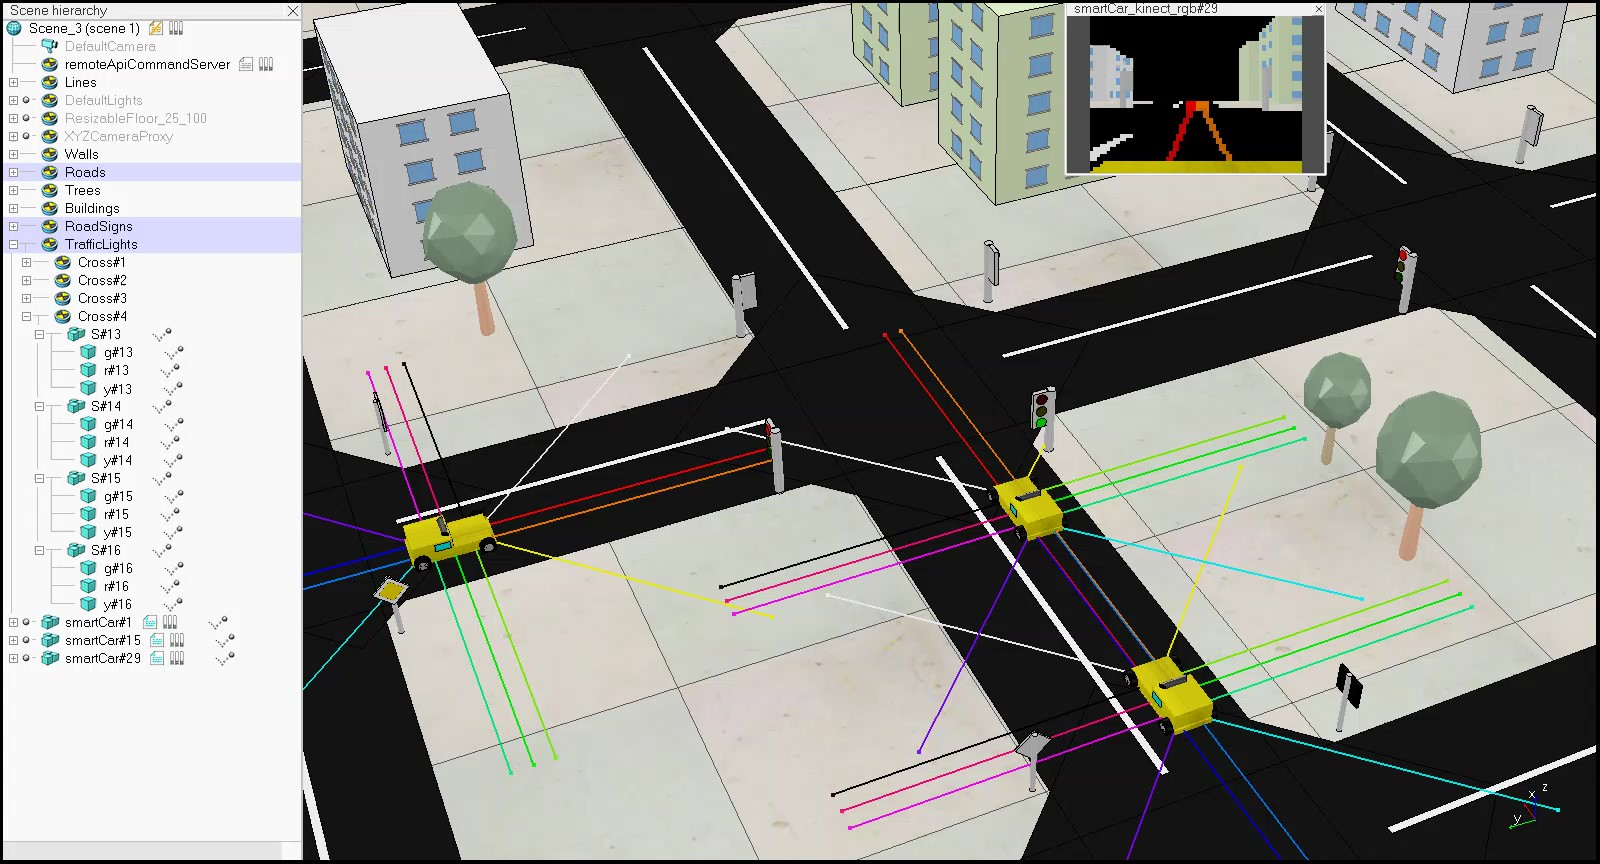
\includegraphics[width=.7\linewidth]{p11.jpg}
	\caption{Początek symulacji - scen. 1}
	\label{fig:p11}
\end{figure} \vspace{-0.5cm}

\begin{figure}[H]
	\centering
	\centering
	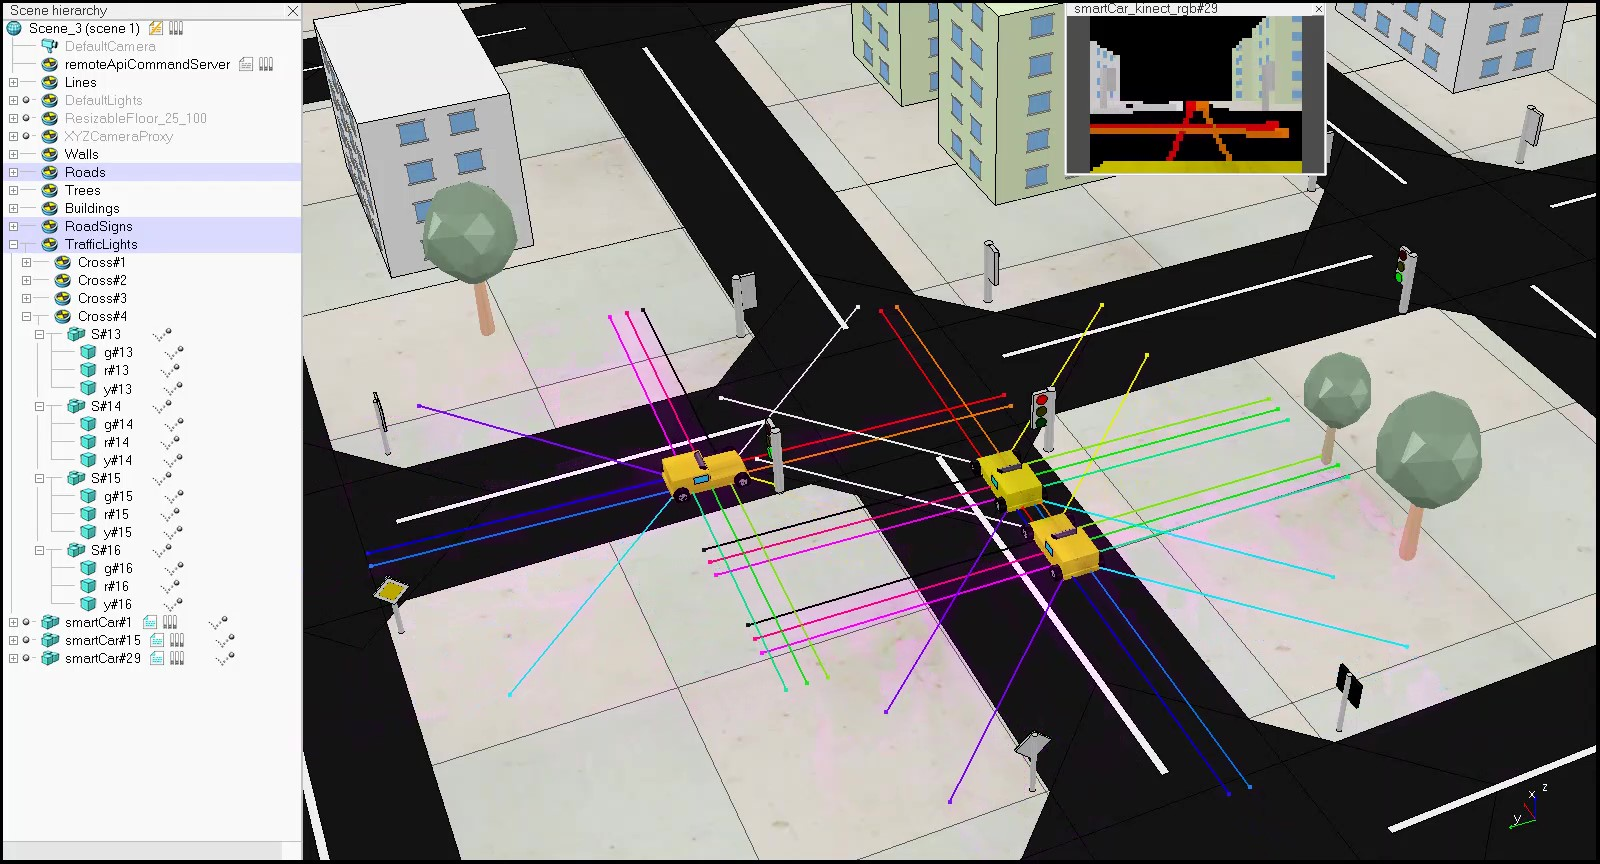
\includegraphics[width=.7\linewidth]{p12.jpg}
	\caption{Wykrycie kolizji po dojeździe do skrzyżowania - scen. 1}
	\label{fig:p12}
\end{figure}

\subsection{Scenariusz 2 -- pokonywanie skrzyżowań}

W drugim scenariuszu zbadano zdolność pojazdów do pokonywania skrzyżowań. Samochody pokonywały skrzyżowania zgodnie z pierwszeństwem wyznaczanym przez zawczasu ustalony priorytet dróg. Samochody zatrzymywały się przed skrzyżowaniem w momencie gdy na drodze o wyższym priorytecie znajdowały się samochody zbliżające się do skrzyżowania. Przykładowe migawki z symulacji przedstawiono poniżej.

\begin{figure}[H]
	\centering
	\centering
	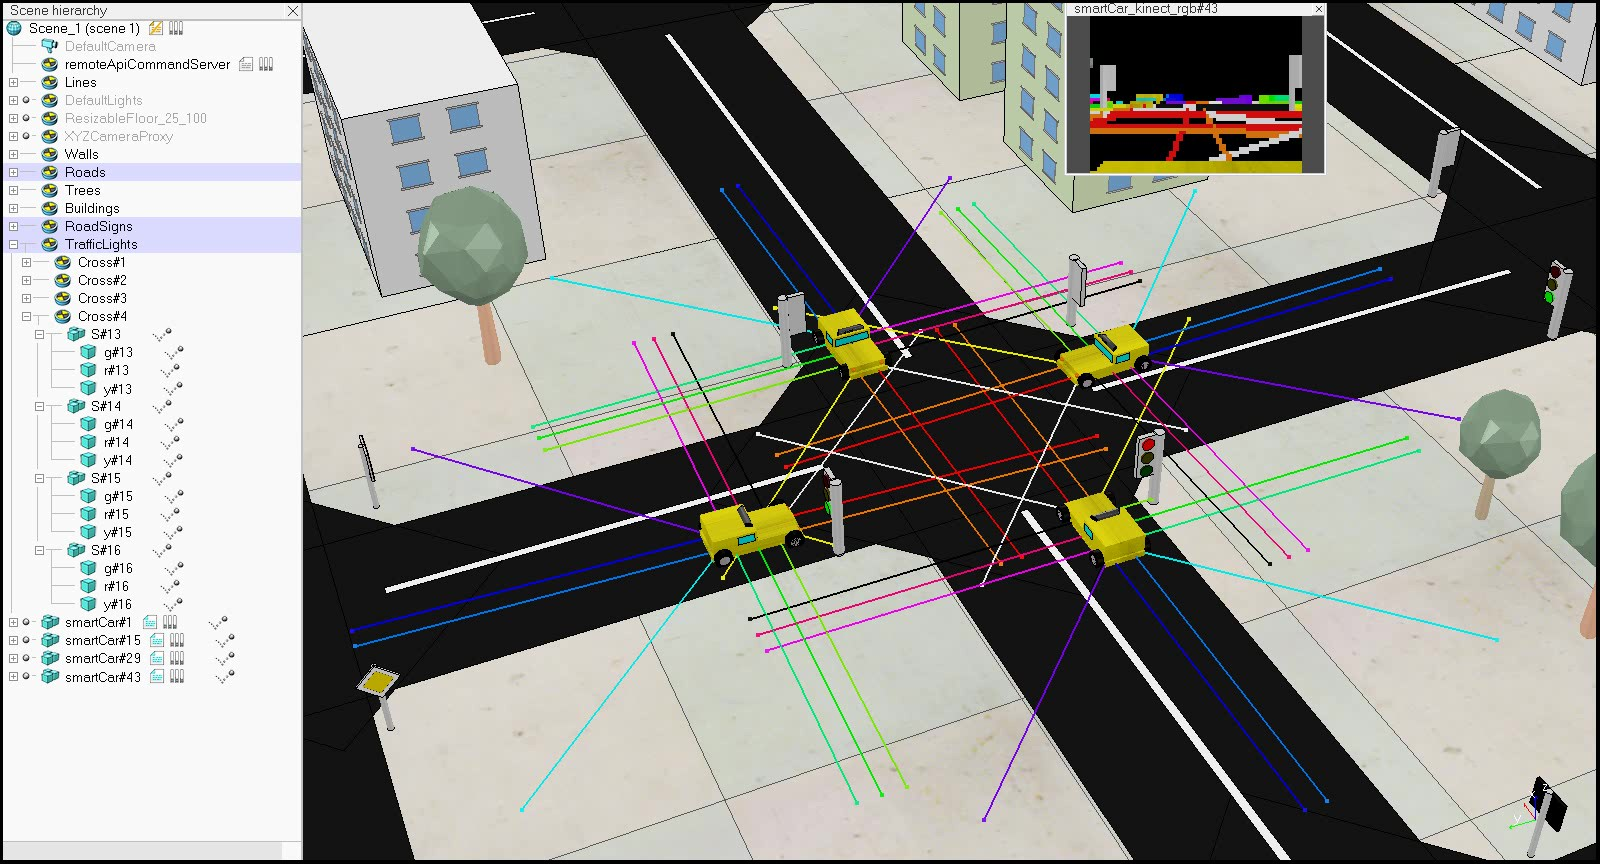
\includegraphics[width=.8\linewidth]{p21.jpg}
	\caption{Początek symulacji - scen. 2}
	\label{fig:p21}
\end{figure}

\begin{figure}[H]
	\centering
	\centering
	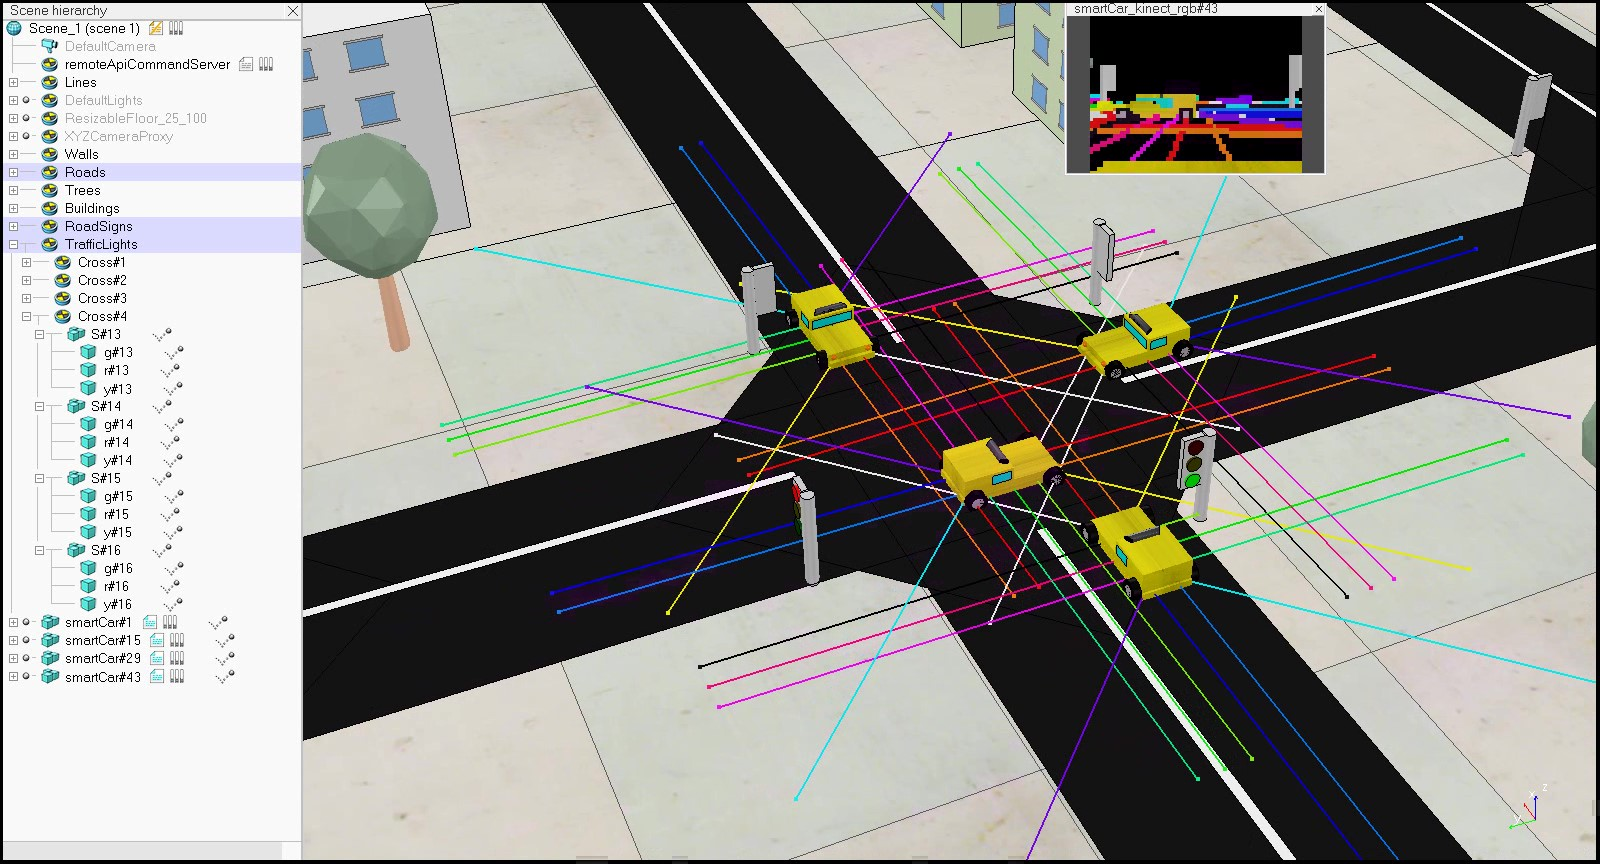
\includegraphics[width=.8\linewidth]{p22.jpg}
	\caption{Przejazd 1. samochodu przez skrzyżowanie - scen. 2}
	\label{fig:p22}
\end{figure}

Można zauważyć, że samochody pokonują skrzyżowania w~określonym porządku, zgodnie z~priorytetyzacją dróg. W~przypadku dalszego rozwoju projektu można by zasymulować bardziej realistyczne warunki związane ze~zmianą sygnalizacji świetlnej oraz z~uwzględnieniem zróżnicowanych znaków drogowych. 

\begin{figure}[H]
	\centering
	\centering
	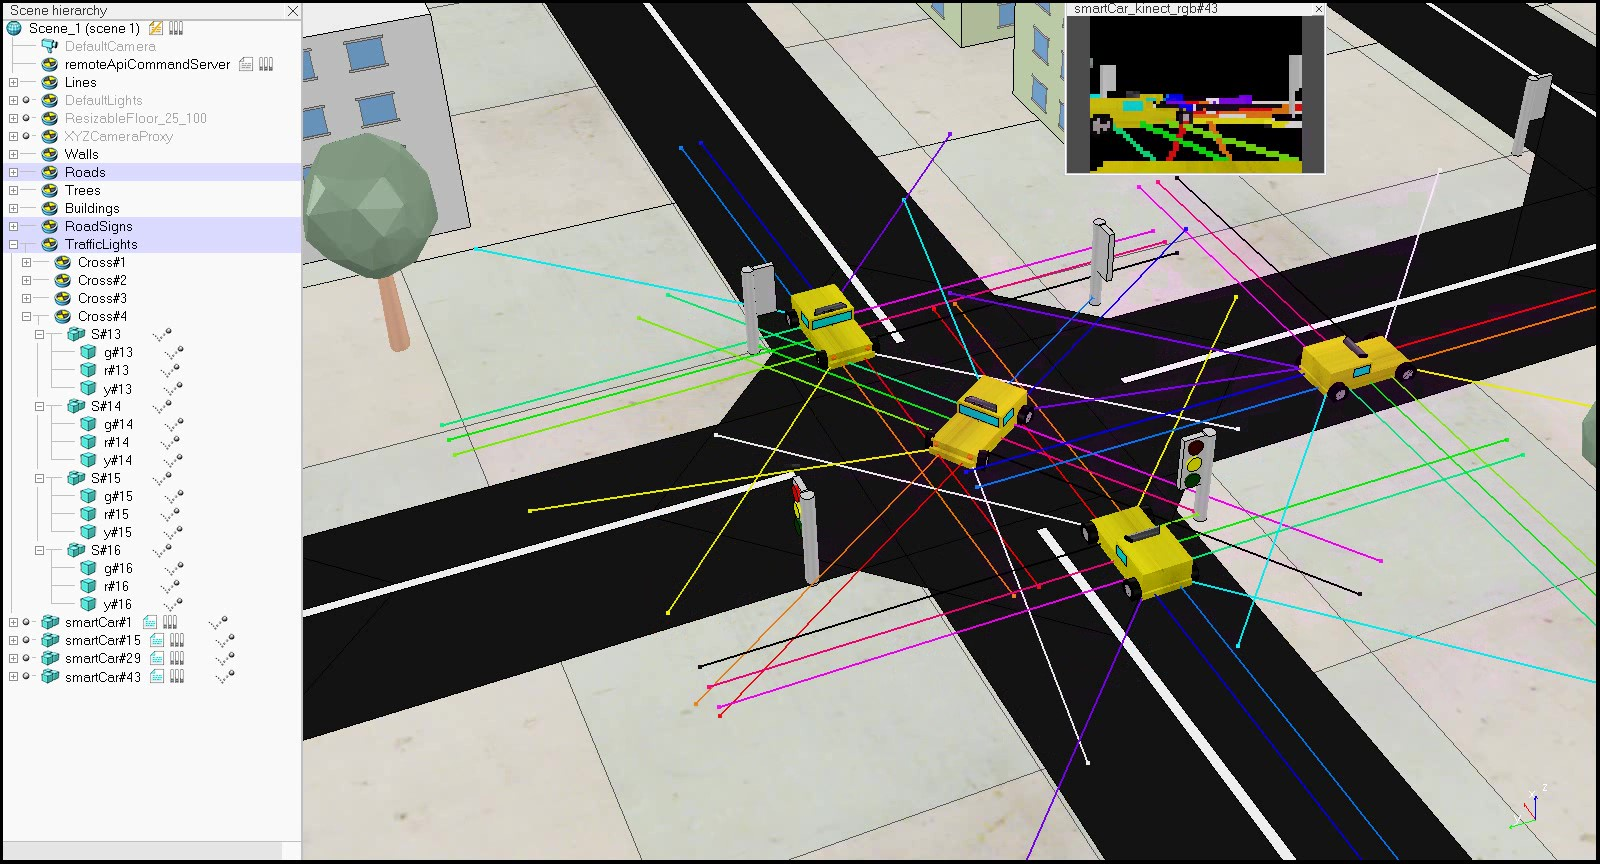
\includegraphics[width=.8\linewidth]{p23.jpg}
	\caption{Skręt w lewo 2. samochodu przez skrzyżowanie - scen. 2}
	\label{fig:p23}
\end{figure}

\begin{figure}[H]
	\centering
	\centering
	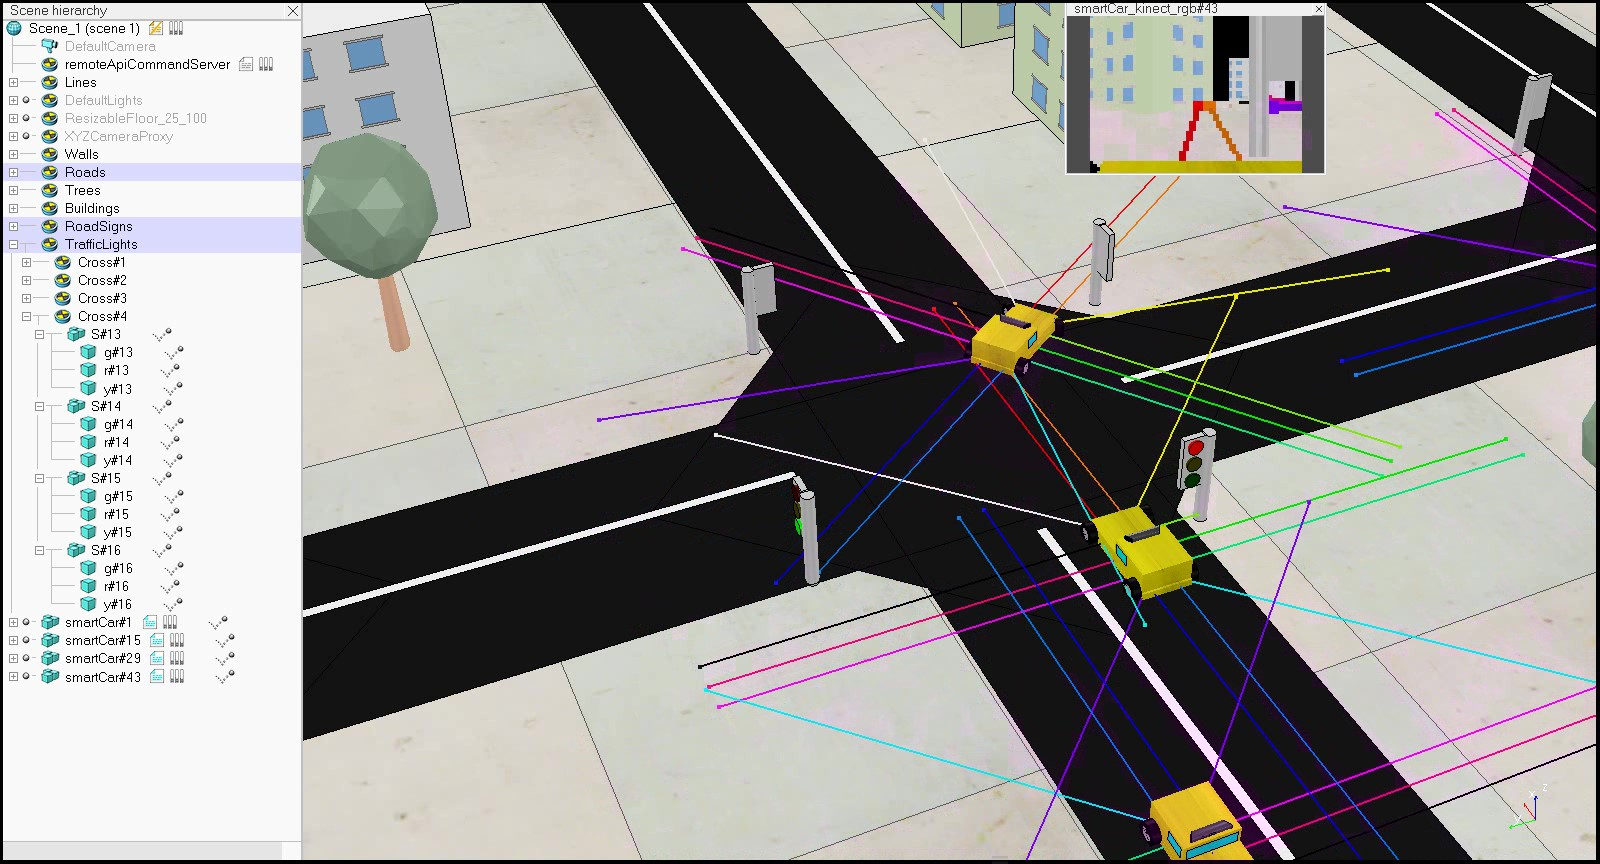
\includegraphics[width=.8\linewidth]{p24.jpg}
	\caption{Zawracanie 3. samochodu na skrzyżowaniu - scen. 2}
	\label{fig:p24}
\end{figure}

\begin{figure}[H]
	\centering
	\centering
	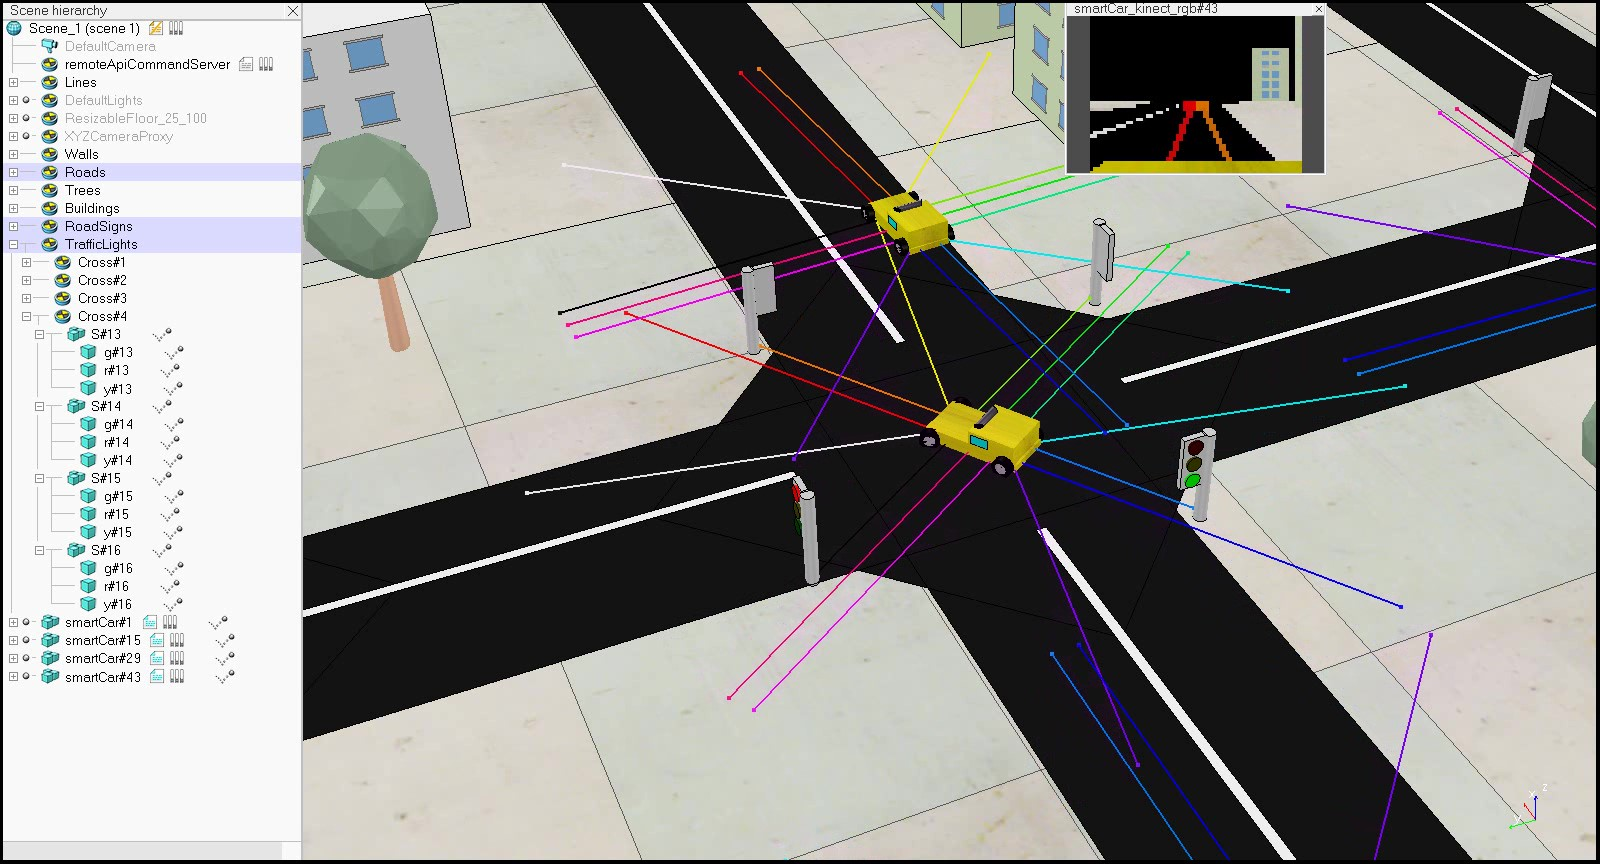
\includegraphics[width=.8\linewidth]{p25.jpg}
	\caption{Zawracanie 4. samochodu na skrzyżowaniu - scen. 2}
	\label{fig:p25}
\end{figure}

\subsection{Scenariusz 3 -- przejazd pojazdów do punktów docelowych}
 
W ostatnim scenariuszu zbadano zdolność pojazdów do pokonywania zadanych tras w obliczu dużego ruchu. Przeprowadzono symulację z 8 samochodami, którym punkty docelowe zadano w~sposób losowy. Przykładowe migawki z symulacji przedstawiono poniżej.
  
Okazuje się, że pojazdy poradziły sobie z~dotarciem do~położeń docelowych, a~jednocześnie uniknęły kolizji. Główne aspekty symulatora zostały w~ten sposób przetestowane. Oczywiście w~razie dalszego rozwoju można by się pokusić o~przeprowadzenie bardziej specjalistycznych symulacji pod~względem ich zgodności z~warunkami rzeczywistymi.

 \begin{figure}[H]
 	\centering
 	\centering
 	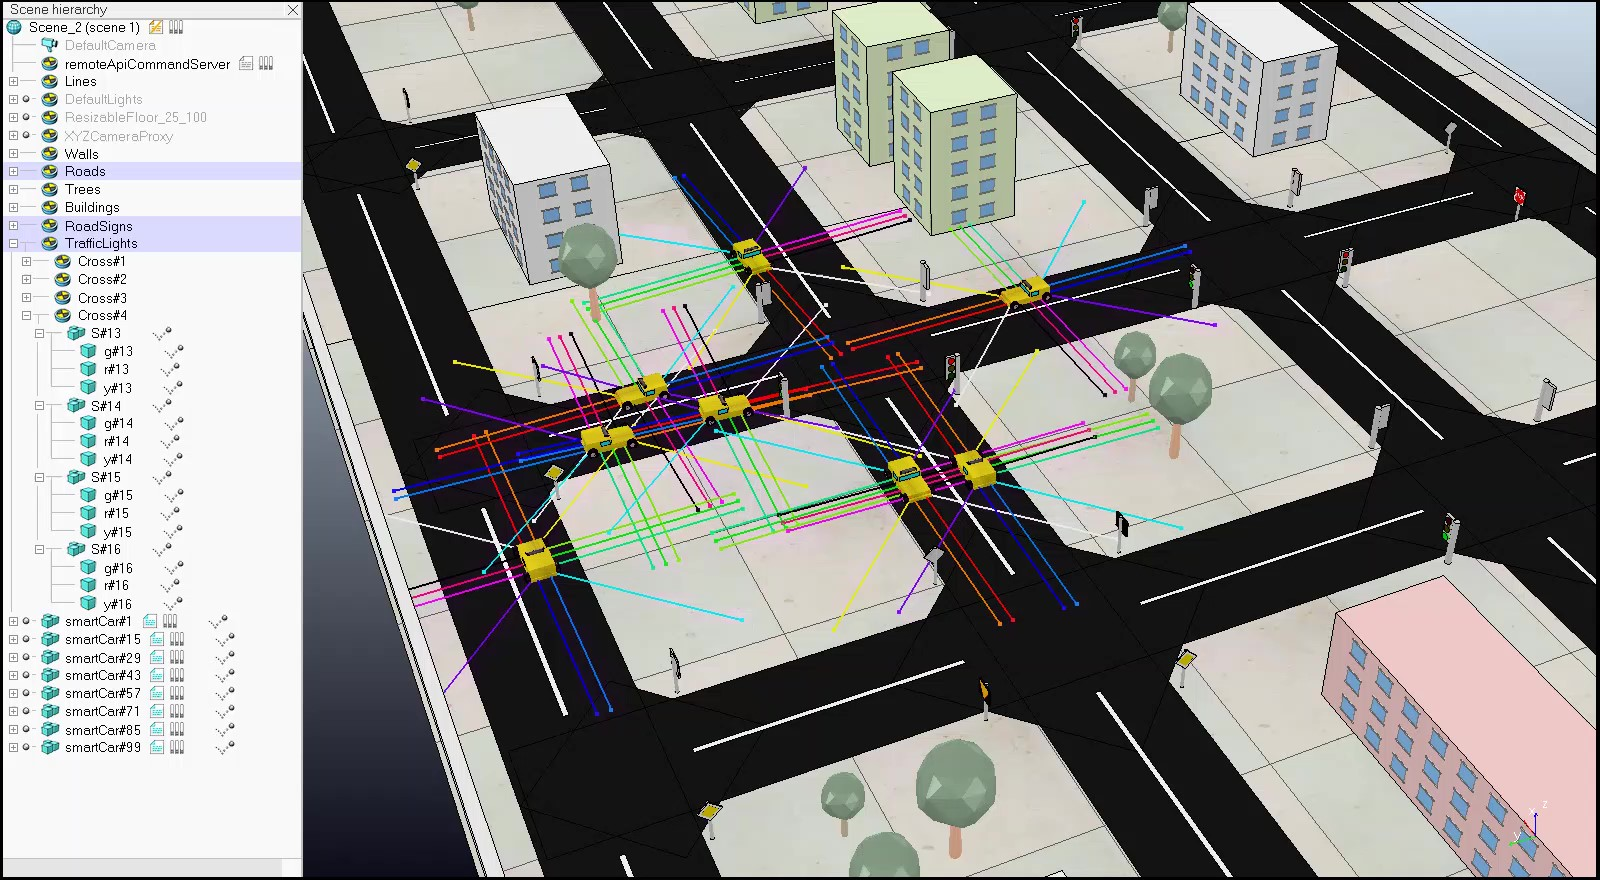
\includegraphics[width=.8\linewidth]{p31.jpg}
 	\caption{Początek symulacji - scen. 3}
 	\label{fig:p31}
 \end{figure}

 \begin{figure}[H]
	\centering
	\centering
	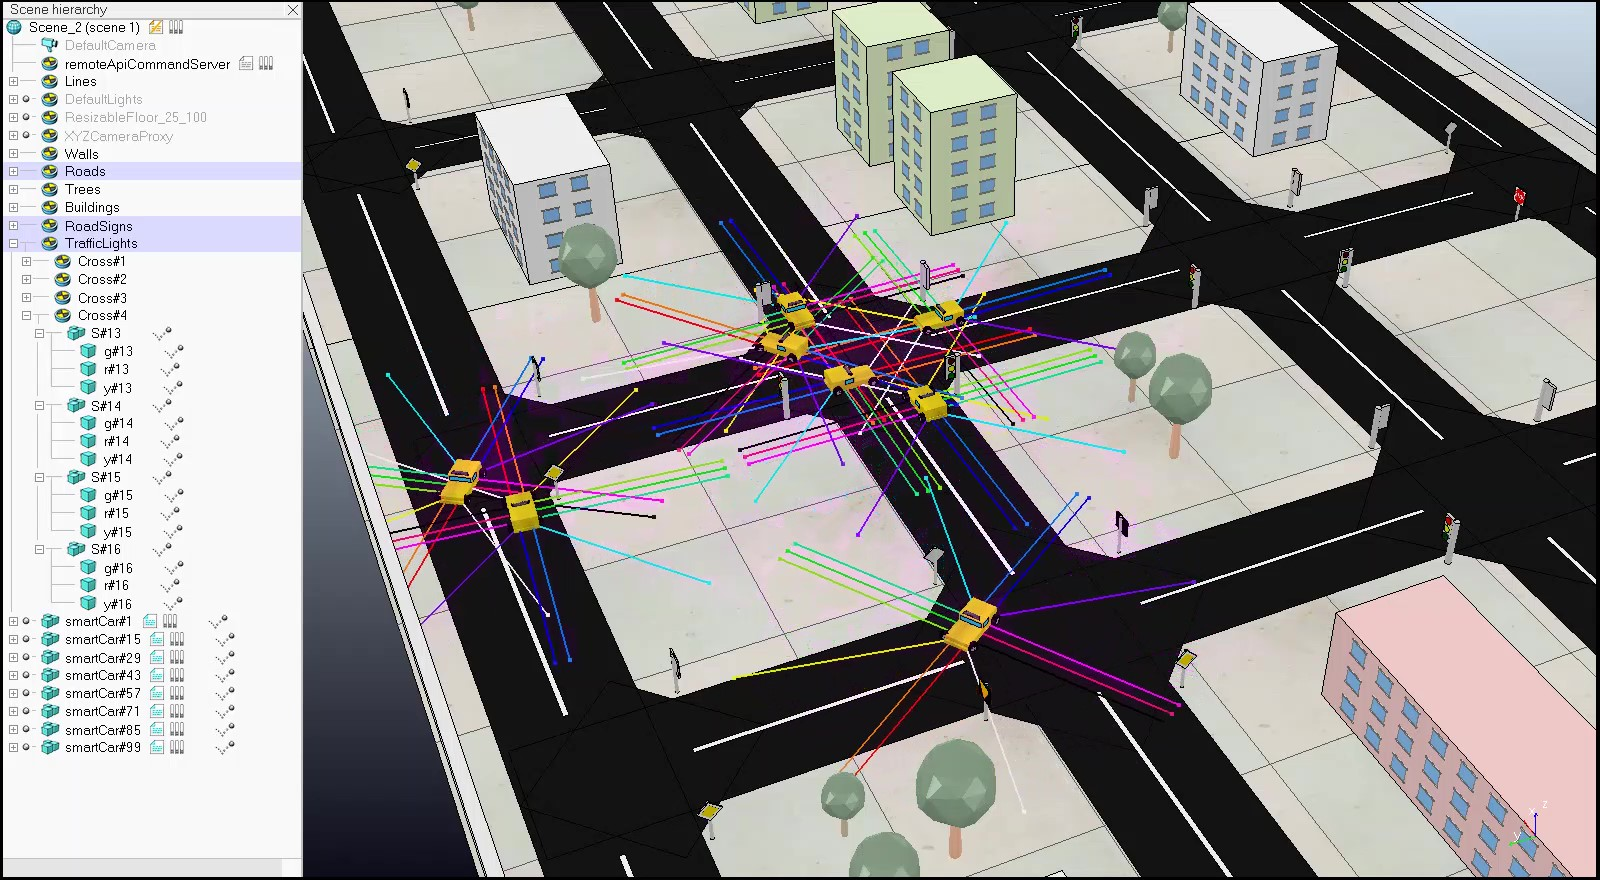
\includegraphics[width=.8\linewidth]{p32.jpg}
	\caption{Migawka z symulacji - scen. 3}
	\label{fig:p32}
\end{figure}

 \begin{figure}[H]
	\centering
	\centering
	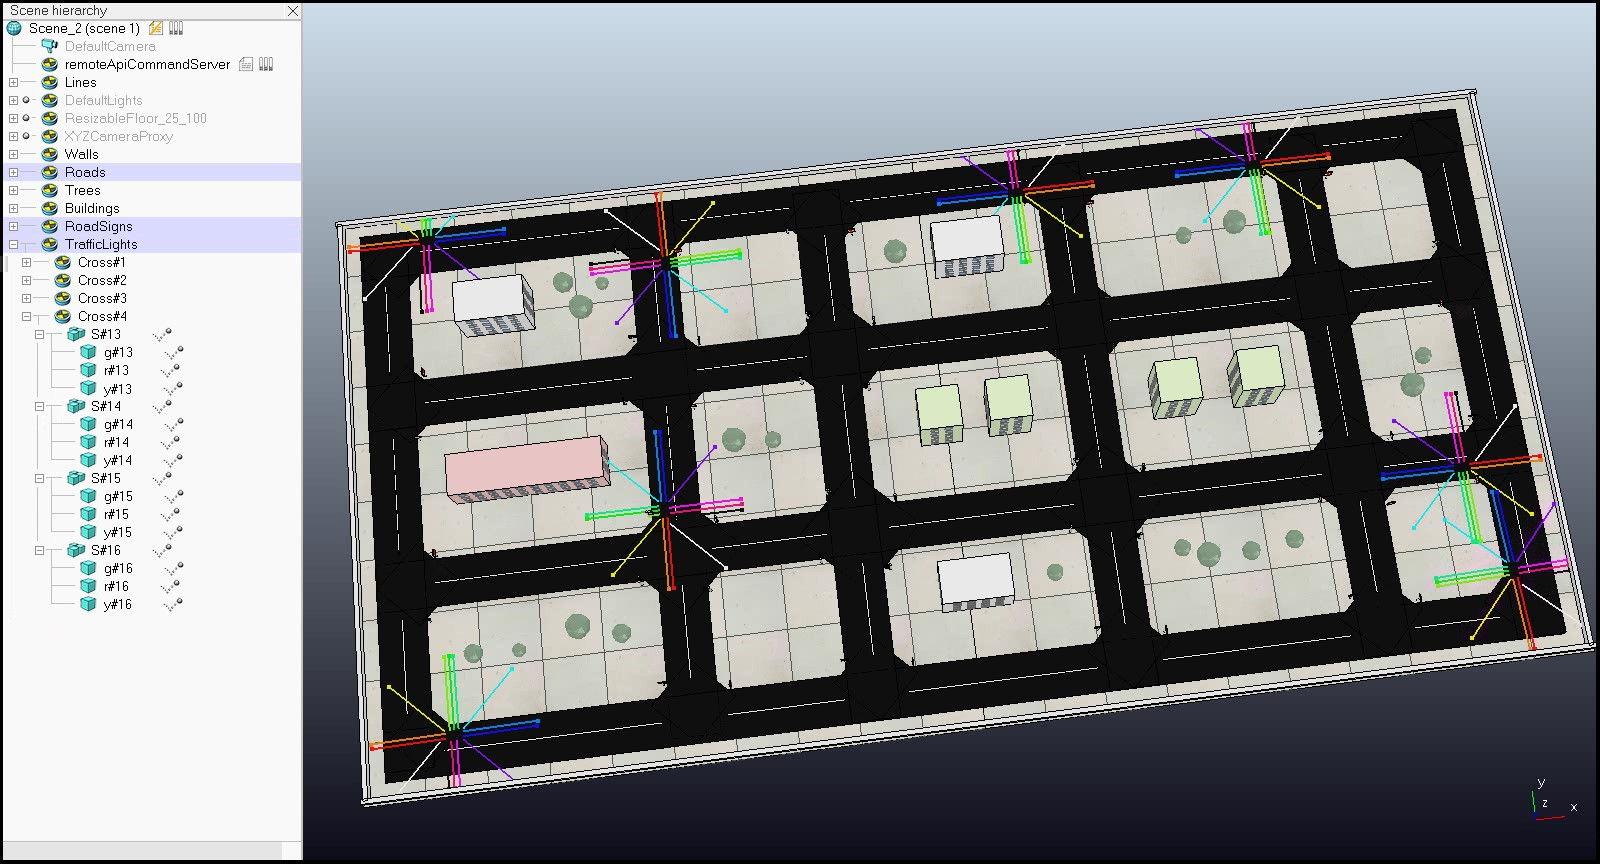
\includegraphics[width=.8\linewidth]{p33.jpg}
	\caption{Koniec symulacji - zaznaczone końcowe pozycje - scen. 3}
	\label{fig:p33}
\end{figure}
 
 
